
\chapter{Vectors}

This chapter covers the following ideas. 

% A list of objectives for the chapter
%\begin{enumerate}
%\item ...
%\end{enumerate}

\begin{enumerate}
\item Define, draw, and explain what a vector is in two and three
  dimensions.
\item Add, subtract, multiply (scalar, dot, and cross product)
  vectors. Be able to illustrate each operation geometrically.
\item Use vector products to find angles, length, area, projections,
  and work.
\item Use vectors to give equations of lines and planes and be able to
  draw lines and planes in 3D.
\end{enumerate}



%%% Local Variables: 
%%% mode: latex
%%% TeX-master: "../multivariable-calculus"
%%% End: 


\section{Multiple dimensions}
Before plotting points in three dimensions, we need to establish
conventions about the axes. The most common method of graphing is to
use a right-hand coordinate system.  Your right pointer finger
represents the positive {$x$}-axis, your middle finger represents the
positive {$y$}-axis, and your thumb represents the positive
{$z$}-axis.  Your hand represents the origin (the point $(0,0,0)$).
To plot a point in 3D, it's helpful to visualize a rectangular box
with one corner at the origin and the opposing corner at the point of
interest.

%\begin{example}
%  \note{plot the boxes representing (1,2,3) and (-1,4,-2)}
%\end{example}

We use the Pythagorean theorem twice to find distances in three
dimensions.  To find the distance between the origin and a point
$(x,y,z)$, the Pythagorean theorem gives the distance from {$(0,0,0)$}
to {$(x,y,0)$} as {$\sqrt{x^2+y^2}$}.  The length of the hypotenuse of
the triangle with vertices $(0,0,0)$, $(x,y,0)$, and $(x,y,z)$ is
hence $\sqrt{(\sqrt{x^2+y^2})^2+z^2} = \sqrt{x^2+y^2+z^2}$.  This
formula generalizes to show that the distance between two points is
$\sqrt{(x_2-x_1)^2+(y_2-y_1)^2+(z_2-z_1)^2}$.

\begin{example}
  The distance from the origin to ($3,5,-2)$ is
  {$\sqrt{(3)^2+(5)^2+(-2)^2} = \sqrt{9+25+4} = \sqrt{38}$}.

  The distance between $P_1=(1,0,2)$ and $P_2=(3,1,0)$ is
  $\sqrt{(3-1)^2+(1-0)^2+(0-2)^2} = 3$.
\end{example}

In addition, since a sphere of radius $r$ centered at $(x_0,y_0,z_0)$ is
defined as all points $(x,y,z)$ which are distance $r$ from the
center, we get (by squaring both sides of the distance formula) that
the equation of a sphere is $(x-x_0)^2+(y-y_0)^2+(z-z_0)^2 = r^2$.

\begin{example}
  The equation $x^2+y^2+z^2+2x-4y = 0$ can be rewritten (by completing
  the square) as $x^2+2x+1+y^2-4y+4+z^2=1+4$ or
  $(x+1)^2+(y-2)^2+z^2=5$, so it is a sphere of radius $\sqrt 5$
  centered at $(-1,2,0)$.
\end{example}

We will focus most of our time this semester on two- and
three-dimensional problems. However, many problems in the real world
require a higher number of dimensions. When you hear the word
``dimension'', it does not always represent a physical dimension, such
as length, width, or height.  If a quantity depends on 30 different
measurements, then the problem involves 30 dimensions.  As a quick
illustration, the formula for the distance between two points depends
on 6 numbers, so distance is really a 6-dimensional problem.  As
another example, if a piece of equipment has a color, temperature,
age, and cost, we can think of that piece of equipment being
represented by a point in four-dimensional space (where the coordinate
axes represent color, temperature, age, and cost).

\section{Vectors}
A vector (written $\vec v$ or in bold face $\mathbf{v}$) is a
magnitude in a certain direction. Vectors are used to represent
forces, velocity, acceleration, and many other quantities. One useful
way to visualize a vector is as an arrow pointing in a certain
direction with a certain length (magnitude).  
The part of the arrow
with the arrowhead is called the ``head'' of the arrow or vector,
while the other end is the ``tail''.  Two vectors are equal if they
both represent the same magnitude in the same direction, regardless of
where the vectors are drawn.
{\marginpar{{
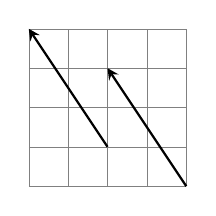
\begin{tikzpicture}[scale=.5]
\draw[help lines,step=1cm] (0,0) grid (4,4);
\draw[->,>=stealth,thick] (2,1) -- (0,4);
\draw[->,>=stealth,thick] [xshift=2cm, yshift=-1cm](2,1) -- (0,4);
\end{tikzpicture}

Both vectors 
represent $\left<-2,3\right>$, regardless of where they start.
}}}



The vector which points one unit in the $x$ direction is written in
one of the three ways, $\ii = \vec \imath= \langle1,0,0\rangle$. Similarly we define
$\jj = \vec \jmath= \langle0,1,0\rangle$ and $\kk = \vec k = \langle0,0,1\rangle$. It is also
common to write vectors in parentheses instead of angle brackets.

Vectors are often drawn with their tail at the origin and the head at
the coordinates specified. The component form of a vector $\vec v$
centered at the origin with head at $(v_1,v_2,v_3)$ can be written
as $\langle v_1,v_2,v_3\rangle$, $(v_1,v_2,v_3)$, or $v_1\ii+v_2\jj+v_3\kk$. Since it is rather
difficult to write in bold face font on paper, we will write vectors
with an arrow above them and we will use the forms $\langle
v_1,v_2,v_3\rangle$ or $(v_1,v_2,v_3)$ much
more often than $v_1\ii+v_2\jj+v_3\kk$ because it takes less space.

		
\section{Vector Arithmetic}
We add and subtract vectors component-wise. To multiply a vector by a
scalar, multiply each component by the scalar.  
\begin{example}
$\langle1,3\rangle-2\langle-1,2\rangle+\langle4,0\rangle = \langle1-2(-1)+4,3-2(2)+0\rangle = \langle7,-1\rangle$  
On paper it is often convenient to write vectors using column notation
as in
$$\colvec{1\\3}-2\colvec{-1\\  2} + \colvec{4\\0} 
= \colvec{1-2(-1)+4\\3-2(2)+0} = \colvec{7\\-1}.$$ 
\end{example}
Vector addition can be performed geometrically by placing the tail of
the second vector at the head of the first. The resultant vector is
the vector which starts at the tail of the first and ends at the head
of the second. This is called the parallelogram law of
addition. Scalar multiplication is equivalent to stretching a vector
by the scalar, and if the scalar is negative, then the vector reverses
to point in the opposite direction.

These arithmetic operations are illustrated geometrically below. Take
some time to practice drawing vectors and performing addition,
subtraction, and scalar multiplication geometrically. Notice that
vector subtraction $\vec u - \vec v$ yields a vector whose head is at
the head of $\vec u$ and tail at the head of $\vec v$.  I remember
this by visualizing subtraction as $\vec u \gets \vec v$.
  \begin{center}
  \begin{tabular}[c]{ccc}
    \begin{tikzpicture}
      \draw [grid lines] (0,0) grid (4,3);
      \draw[->] (0,0) -- node[left] {$\vec u$} (1,2);
      \draw[->] (0,0) -- node[below] {$\vec v$} (3,1);
      \draw[->] (1,2) -- node[above] {$\vec v$} (4,3);
      \draw[->,ultra thick] (0,0) -- node[right=3pt] {$\vec u + \vec v$} (4,3);
    \end{tikzpicture}
    

&  

    \begin{tikzpicture}
      \draw [grid lines] (-2,0) grid (3,3);
      \draw[->] (0,0) -- node[left] {$\vec u$} (1,2);
      \draw[->] (0,0) -- node[below] {$\vec v$} (3,1);
      \draw[->] (1,2) -- node[above] {$-\vec v$} (-2,1);
      \draw[->,ultra thick] (0,0) -- node[below left] {$\vec u - \vec v$} (-2,1);
      \draw[->,ultra thick] (3,1) -- node[above right] {$\vec u - \vec v$} (1,2);
    \end{tikzpicture}
&
    \begin{tikzpicture}
      \draw [grid lines] (-1,0) grid (2,3);
      \draw[->] (0,0) -- node[below right] {$\vec u$} (1,1);
      \draw[->] (-1,0) -- node[above left] {$\vec 2u$} (1,2);
      \draw[->] (2,2) -- node[below right] {$-\frac{1}{2} \vec u$} (1.5,1.5);
    \end{tikzpicture}
  \end{tabular}
\end{center}

The magnitude (or length, or absolute value) of a vector is found
using the distance formula. We write $||\vec u|| = |\vec u| =
\sqrt{u_1^2+u_2^2+u_3^2}$, where either double or single bars can be
used. We compute $|\langle1,2,4\rangle| = \sqrt{1+4+16} = \sqrt{21}$. A
unit vector is a vector with magnitude 1. We normalize a vector by
dividing the vector by its magnitude (which makes the vector a unit
vector). Any vector can be written as the product of its magnitude and
a unit vector in the direction of the vector. 

\begin{example}
  We write $\ds
  \langle1,2,4\rangle=\left(\sqrt{21}\right)\left(\frac{\langle1,2,4\rangle}{\sqrt{21}}\right)
  = (\text{magnitude})(\text{unit vector})$. A vector of length 5
  which points in the same direction as $\langle-2,3\rangle$ is $\ds
  (5)\left(\frac{\langle-2,3\rangle}{\sqrt{(-2)^2+3^2}}\right)$.
\end{example}

One of the most important uses of vectors is the idea of a vector
field.  At every point $(x,y)$ in the plane, or $(x,y,z)$ in space, we
place a vector $\vec F (x,y)$, or $\vec F (x,y,z)$ . Two types of
vector fields which occur in nature are radial vector fields and spin
fields.  

		{\psset{unit=.5cm}
\begin{center}
	\begin{tabular}{cc}

    \begin{tikzpicture}[scale=0.5]
      \draw [grid lines] (-2,-2) grid (2,2);
      \draw[->] (1,1) -- (2,2);
      \draw[->] (-1,-1) -- (-2,-2);
      \draw[->] (1,-1) -- (2,-2);
      \draw[->] (-1,1) -- (-2,2);
      \draw[->] (1,0) -- (2,0);
      \draw[->] (0,1) -- (0,2);
      \draw[->] (-1,0) -- (-2,0);
      \draw[->] (0,-1) -- (0,-2);
    \end{tikzpicture}

&
    \begin{tikzpicture}[scale=0.5]
      \draw [grid lines] (-2,-2) grid (2,2);
      \draw[->] (1,0) -- (1,1);
      \draw[->] (-1,0) -- (-1,-1);
      \draw[->] (0,1) -- (-1,1);
      \draw[->] (0,-1) -- (1,-1);
      \draw[->] (1,1) -- (0,2);
      \draw[->] (1,-1) -- (2,0);
      \draw[->] (-1,1) -- (-2,0);
      \draw[->] (-1,-1) -- (0,-2);
    \end{tikzpicture}
\\
{$\vec F(x,y)=\langle x,y\rangle$} (radial vector field)
& 
{$\vec F(x,y)=\langle-y,x\rangle$} (spin field)
	\end{tabular}
\end{center}
		}



\subsection{Dot Product}
The dot product of two vectors $\vec u = \langle u_1,u_2,u_3\rangle$ and
$\vec v =\langle v_1,v_2,v_3\rangle$ is the scalar $\vec u\cdot \vec v =
u_1v_1+u_2v_2+u_3v_3$, and it is defined in other dimensions
similarly.  

\begin{enumerate}
\item Using the law of cosines (and vector subtraction), it can be
  shown that if $\theta$ is the angle between $\vec u$ and $\vec v$, then
  $\ds \cos\theta = \frac{\vec u \cdot \vec v }{|\vec u||\vec v|}$, which means
  that the dot product $\vec u\cdot \vec v = |\vec u||\vec v|\cos\theta$ is
  zero if and only if the angle between $\vec u$ and $\vec v$ is 90
  degrees or $\pi/2$. Two vectors are said to be \emph{orthogonal} if
  the angle between them is $\pi/2$. If $0\leq\theta<\pi/2$, the dot product is
  positive. If $\pi/2<\theta\leq\pi$, the dot product is negative.  The vectors
  $\langle1,3,-2\rangle$ and $\langle4,0,2\rangle$ are orthogonal because the dot product
  $\langle1,3,-2\rangle\cdot \langle4,0,2\rangle=1(4)+3(0)-2(2)$ is zero.

\item In addition to helping understand angles, the dot product helps
  find magnitude, since $\vec u\cdot \vec u = |\vec u| |\vec u| \cos 0 =
  |\vec u|^2$. In high dimensions, the dot product is used to define
  length and angles.

\item The projection of $\vec u$ onto the vector $\vec v$, written
  $\text{proj}_{\vec{v}}\vec{u}$ is a vector parallel to $\vec v$
  whose magnitude is the component of $\vec u$ in the direction of
  $\vec v$.  If you draw both vectors with their base at the origin,
  and create a right triangle with $\vec u$ as the hypotenuse, and the
  adjacent edge on the line containing $\vec v$, then
  $\text{proj}_{\vec{v}}\vec{u}$ is the vector which starts at the
  origin and forms the adjacent side of the triangle.  You can imagine
  $\proj_{\vec v}\vec u$ as the ``shadow'' of $\vec u$ on the line in
  the direction of $\vec v$.

\begin{center}
    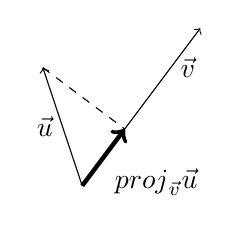
\begin{tikzpicture}[scale=0.5]
      \draw[->] (0,0) -- node[right,near end] {$\vec v$}(3,4);
      \draw[->] (0,0) -- node[left] {$\vec u$} (-1,3);
      \draw[dashed] (-1,3) -- (1.08,1.44);
      \draw[->,ultra thick] (0,0) -- node[below right] {$\text{proj}_{\vec v} \vec u$} (1.08,1.44);
    \end{tikzpicture}
\end{center}
	
The length of the projection is $\ds|\vec u| \cos \theta = |\vec
u|\frac{\vec u\cdot \vec v}{|\vec u||\vec v|} = \frac{\vec u\cdot \vec
  v}{|\vec v|}$. This quantity is called the scalar projection of
$\vec u$ on $\vec v$. A unit vector for the direction of the
projection is $\ds\frac{\vec v}{|\vec v|}$.  Hence we have
$\ds\text{proj}_{\vec v}\vec u = \left(\frac{\vec u\cdot \vec v}{|\vec
    v|}\right)\frac{\vec v}{|\vec v|}$, and the scalar projection of
$\vec u$ on $\vec v$ is {$\displaystyle |\vec{u}| \cos\theta =
  \frac{\vec{u}\cdot \vec{v}}{|\vec{v}|}$}.

\item
When a force $\vec F$ and a displacement $\vec d$ are in the same
direction, we define the work done by $\vec F$ acting through a
displacement $\vec d$ to be $W=|\vec F||\vec d|$ (force times
displacement). However if the force and displacement are in different
directions, then we find the portion of work parallel to the direction
of displacement (the component of $\vec F$ in the direction of $\vec
d$) and use that quantity to compute work $W=|\vec F|\cos\theta |\vec d|$.
This simplifies to become simply $W=\vec F\cdot \vec d$.

If an object moves from the point $(0,3)$ to the point $(6,0)$, the
work done by the force {$\vec F = \langle0,-200\rangle$} acting through
that displacement is $W=\langle0,-200\rangle\cdot \langle6,-3\rangle = 600$.

\item 
Notice that in finding work, we use the portion of $\vec F$ parallel
to $\vec d$ to compute work.  The portion of $\vec F$ orthogonal to
$\vec d$ contributes nothing to the work done. It is often useful to
be able to write a vector $\vec F$ as the sum of a vector parallel to
$\vec d$ and a vector orthogonal to $\vec d$.  The formula is $\vec F
= \text{proj}_{\vec d}\vec F + (\vec F - \text{proj}_{\vec d}\vec F)$.  

\begin{example}
  $\text{proj}_{\langle6,-3\rangle}\langle0,-200\rangle =
  \frac{\langle0,-200\rangle\cdot\langle6,-3\rangle
  }{|\langle6,-3\rangle|}\frac{\langle6,-3\rangle}{|\langle6,-3\rangle|}
  = \frac{600}{45}\langle6,-3\rangle =\langle80,-40\rangle$, so we
  can write $\vec F = \langle0,-200\rangle = \langle80,-40\rangle
  +\left(\langle0,-200\rangle-\langle80,-40\rangle \right) =
  \langle80,-40\rangle + \langle-80,-160\rangle.$ Work can be found by
  looking at the parallel part, as $W=\left(\langle80,-40\rangle +
    \langle-80,-160\rangle\right)\cdot \langle6,-3\rangle =
  \langle80,-40\rangle \cdot \langle6,-3\rangle +0 = 600$.
\end{example}
\end{enumerate}




\subsection{Cross Product}
The cross product of two vectors $\vec u = \langle u_1,u_2,u_3\rangle$
and $\vec v = \langle v_1,v_2,v_3\rangle$ is a new vector $$\vec u\times \vec
v = \langle u_2v_3-u_3v_2,-(u_1v_3-u_3v_2),u_1v_2-u_2v_1\rangle =
\det\begin{bmatrix}\vec i & \vec j&\vec k\\ u_1&u_2&u_3\\
v_1&v_2&v_3\\\end{bmatrix}.$$

\begin{enumerate}
\item
The cross product of two vectors is a new vector which is orthogonal
to both $\vec u$ and $\vec v$. This can be checked by performing the
dot products $\vec u \cdot (\vec u \times \vec v)$ and $\vec v \cdot (\vec u \times \vec
v)$. 

\item

It can be shown that the magnitude of the cross product is {$|\vec u \times
\vec v| = |\vec u||\vec v|\sin\theta$}, which is very similar to the dot
product, but it involves a $\sin\theta$ instead of $\cos\theta$. Using this
formula, the magnitude of the cross product is the area of the
parallelogram formed using the two vectors $\vec u$ and $\vec v$.

\begin{center}
    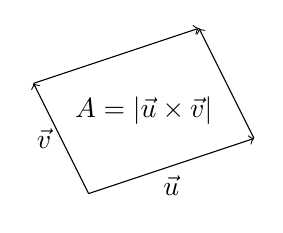
\begin{tikzpicture}[scale=0.7]
      \draw[->] (0,0) -- node[below] {$\vec u$} (3,1);
      \draw[->] (0,0) -- node[left] {$\vec v$} (-1,2);
      \draw[->] (-1,2) -- (2,3);
      \draw[->] (3,1) -- (2,3);
      \node at (1,1.5) {$A=|\vec u \times\vec v|$};
    \end{tikzpicture}
\end{center}

\item Since the cross product is orthogonal to both $\vec u$ and $\vec
v$, it must point in one of two directions. The direction of the cross
product is found using the right hand rule. If you place your right
index finger on the vector $\vec u$, and then rotate your hand so that
your middle finger is in the direction of $\vec v$, then the direction
of $\vec u\times\vec v$ is in the direction of your thumb. 

\item Note that {$\vec u\times \vec v = - \vec v\times \vec u$}. Because of
this, we say the cross product is anti commutative, so be careful not
to switch the order on the cross product. 

\item Other applications of the cross product involve finding the
volume of a parallelepiped and torque.

\end{enumerate}

A vector which is orthogonal to both $\langle1,-2,3\rangle$ and
$\langle2,0,-1\rangle$  is 
\begin{align*}
  \langle1,-2,3\rangle\times \langle2,0,-1\rangle &=
  \det\begin{bmatrix}\vec i & \vec j&\vec k\\ 1&-2&3\\
    2&0&-1\\\end{bmatrix} \\
  &= \langle(-2)(-1)-(0)(3),-[
  (1)(-1)-(2)(3)],(1)(0)-(2)(-2)\rangle \\
  &= \langle2,7,4\rangle.
\end{align*}
Notice that if I reverse the order, then $\langle2,0,-1\rangle \times\langle1,-2,3\rangle =
-\langle2,7,4\rangle$ is also orthogonal to both $\langle1,-2,3\rangle$ and $\langle2,0,-1\rangle$, it
just points in the opposite direction. In addition, the area of the
parallelogram formed by the vectors $\langle1,-2,3\rangle$ and $\langle2,0,-1\rangle$ is
$|\langle2,7,4\rangle| = \sqrt{4+49+16}=\sqrt{69}$.










\section{Lines and planes}
\subsection{Lines}
Back in college algebra, or high school, we wrote the equation of a
line as {$y=mx+b$}.  The slope, {$m$}, tells us a direction. In vector
form, the slope tells us that the line follows the direction vector
{$\vec v = \langle1,m\rangle$} (one unit increase in $x$ results in an
increase of $m$ units in the $y$ direction). The {$y$}-intercept,
{$b$}, gives us a starting point $(0,b)$ (or written as a vector
{$\vec{r}_0 = \langle0,b\rangle$}) in the plane from which to begin our
graph. In vector form, an equation of the line $y=mx+b$ can be written
as $$\vec r(t) = \langle x,y\rangle =\langle1,m\rangle t
+\langle0,b\rangle= \colvec{1\\m} t
+\colvec{0\\b} = \vec v t+ \vec{r}_0.$$
To find a vector equation of a line in any dimension, you need a
direction vector $\vec v$ and a point $P$ on the line, which we
convert to a vector and call $\vec{r}_0$. A vector equation is then
given by $\vec r(t) = \vec v t+ \vec{r}_0$.

We find the direction vector for the line which passes through the
points $P(1,2,3)$ and $Q(0,-1,4)$ by subtracting the two points, so
$\vec{PQ} = \langle0-1,-1-2,4-3\rangle = \langle-1,-3,1\rangle$. Using
either point, we get two equations of the line as $\vec r_1(t) =
\langle-1,-3,1\rangle t+ \langle1,2,3\rangle =
\langle-t+1,-3t+2,t+3\rangle$, or $\vec r_2(t) = \langle-1,-3,1\rangle
t+ \langle0,-1,4\rangle = \langle-t,-3t-1,t+4\rangle$.  
To find an equation of the line parallel to $\vec r(t) =
\langle3t,-5t+2,8t-7\rangle$ which passes through the point $(2,-8,1)$,
we need a direction vector and a point.  The direction vector is
parallel to the direction vector of the given line, so we use $\vec v
= \langle3,-5,8\rangle$. The point was given to us as $(2,-8,1)$, so an
equation of the line is $\vec l (t) = \langle3t+2,-5t-8,8t+1\rangle$. 
(I used $l$ instead of $r$ because $r$ was already used.)
 
Two other ways to write the equation of a line are \emph{parametric
  equations} and \emph{symmetric equations}.  If a line has the vector
equation $\langle-t, -3t-1,2t+4\rangle$, then the parametric equations are simply
\begin{equation*}
  x=-t, \quad y=-3t-1, \quad z=2t+4.
\end{equation*}
The symmetric equations are found by solving for $t$ in each of the
above equations and setting pairs equal to each other, like this:
\begin{equation*}
  -x=\frac {y+1}{-3},\quad -x=\frac {z-4}{2}, \quad \frac{y+1}{-3}=\frac{z-4}{2}.
\end{equation*}
These three equations can be written more compactly as $\ds
  -x=\frac {y+1}{-3}=\frac {z-4}{2}$.
Note that you cannot write the symmetric equations if, for example,
$x=3$ is one of the parametric equations (you'd be dividing by zero then).

\subsection{Planes}

We say a vector is normal to a plane if it is orthogonal to every
vector which lies in the plane.  A normal vector ``sticks out'' of a
plane. If you have a point {$P(a,b,c)$} on a plane, and  a vector
{$\vec n = \langle A,B,C\rangle$} normal to the plane, then for any
point $Q(x,y,z)$ in the plane, the vector
$\vec{PQ}=\langle x-a,y-b,z-c\rangle$ is a vector in the plane, hence
orthogonal to $\vec n$. This gives the following as equations of the
plane: 
$$
\begin{array}{rl}\vec n \cdot \langle x-a,y-b,z-c\rangle &= 0\\
\langle A,B,C\rangle \cdot \langle x-a,y-b,z-c\rangle &= 0\\
A(x-a)+B(y-b)+C(z-c)&= 0\\
Ax+By+Cz&= D
\end{array}$$
where $D$ is a constant.  Any equation of the form $Ax+By+Cz= D$ is an
equation of a plane with normal vector {$\vec n =
\langle A,B,C\rangle$}. 

A normal vector for the plane which passes through the points
$P(1,0,0)$, $Q(2,0,-1)$, and $R(0,1,3)$ is found using the cross product $\vec n
= \vec{PQ}\times \vec{PR} = \langle1,0,-1\rangle\times\langle-1,1,3\rangle =
\langle1,-2,1\rangle$.  So an equation of the plane can be found by
using $\vec n$ and any of the three points, which yields
$1(x-1)-2(y-0)+1(z-0)=0$, or $x-2y+z=1$.
As a second example, to find a normal vector for the plane containing
the two intersecting lines {$\vec r_1(t) = \langle1+t,3t,2 \rangle$}
and {$\vec r_2(t) = \langle2+2t,3,2-t \rangle$}, compute $\vec n = \vec
v_1\times \vec v_2 = \langle1,3,0\rangle \times \langle2,0,-1\rangle=\langle-3,1,-6
\rangle$. Since the plane contains both lines, we can use any point on
either line as our point.  I will use {$\vec r_1(0) = \langle1,0,2
\rangle$}, and so an equation of the line is
$-3(x-1)+1(y-0)-6(z-2)=0$.

Lastly, if two planes intersect, then they will intersect in a line. 
A direction vector for that line can be found by computing the cross
product of the two normal vectors.  If that cross product is zero,
then the two planes are parallel. Otherwise, you can use the dot
product of the two normal vectors to find the angle of intersection of
the planes.

To sketch a plane, plot 3 non-collinear points. If the plane is
written in the form {$\displaystyle\frac xa+\frac yb+\frac zc=1$},
then the plane passes through the coordinate axes at the points
$(a,0,0),(0,b,0),(0,0,c)$. This is very similar to what happens with
conic sections. Take a moment to sketch the planes {$2x+3y+z=6$},
{$x-4y=8$}, and {$\displaystyle\frac x2+\frac y3+z=1$}.

Using the dot product, cross product, and projections, derive the
following formulas which find distances between points, lines, and
planes. The distance from a point $Q$ to a plane (with normal vector
{$\vec n$} and a point $P$) is given by $|\text{proj}_{\vec n}\vec
{PQ}|$.  The distance from a point $Q$ to a line (with direction
vector $\vec v$ passing through $P$) is $|\vec{PQ}-\text{proj}_{\vec
v}\vec {PQ}|$. The distance from a line (with direction vector $\vec
v_1$ passing through $P_1$) to a line (with direction vector $\vec
v_2$ passing through $P_2$) is $|\text{proj}_{\vec v_1\times\vec v_2}\vec
{P_1P_2}|$. Practice drawing diagrams to illustrate these
relationships.


One of the main points of calculus is to understand curved objects by
approximating them with flat, linear objects and then using limits to
make the approximation exact. We will approximate space curves with
lines. We will approximate surfaces with planes.  Lines and planes are
crucial to generalizing calculus to higher dimensions.






%%% Local Variables: 
%%% mode: latex
%%% TeX-master: "../multivariable-calculus"
%%% End: 





